\chapter{使用方法}
\section{{\tt main.tex}文件}
将文档类选择{\tt ructhesis},文档的选项有{\tt bachelor、master、promaster、doctor}代表不同的学位论文排版方式。\par 
在导言区填写扉页相关信息和摘要关键词(需要在关键词间按照本科或者研究生的规定输入空格)。\par

\begin{longtable}[c]{ll}
\caption{命令(环境)解释}\label{tab:performance}\\
\toprule[1.5pt]
命令(环境) & 意义\\\midrule[1pt]
\endfirsthead
\caption[]{命令(环境)解释(续)}\\
\toprule[1.5pt]
 命令(环境) & 意义\\\midrule[1pt]
\endhead
\hline
\multicolumn{2}{r}{续下页}
\endfoot
\endlastfoot
{\tt \textbackslash maketitle}  & 插入扉页 \\
{\tt \textbackslash originality}  &  插入独创性声明 \\
{\tt \textbackslash authorization}  & 插入授权书\\
{\tt \textbackslash tableofcontents}  & 正文目录 \\
{\tt \textbackslash listoffigures}  & 插图目录 \\
{\tt \textbackslash listoftables}  & 表格目录 \\
{\tt \textbackslash autograph}  & 本科签名\footnote{插入签名,在普通章节文件中插入无限制,但在\tt main.tex\rm 文件插入时被插入的章节不能使用\tt\textbackslash include\rm 命令,需使用\tt\textbackslash input\rm 命令。}  \\
{\tt \textbackslash appendix}  & 附录 \\
{\tt \textbackslash bibliographystyle}  & 参考文献样式 \\
{\tt \textbackslash bibliography}  &参考文献数据库 \\
{\tt \textbackslash addcontentsline}  & 加入目录 \\
{\tt abstractzh}  & 中文摘要环境 \\
{\tt abstracten}  & 英文摘要环境 \\
{\tt acknowledge}  & 致谢环境 \\
\bottomrule[1.5pt]
\end{longtable}
\section{{\tt cover.tex}文件}
在{\tt cover.tex}文件中,可以有博士:doctor,学硕:master,专硕:promaster,本科:bachelor,这几个选项。还有shuji选项用于输出书脊。其中{\tt \textbackslash cover}命令用来生成封皮。在有shuji选项的时候可以利用{\tt \textbackslash covertitle}命令制定书脊文字。需要设置纸张高度为两张A4纸宽度(420mm)再加书脊的宽度,100张A4纸厚度约为1cm\upcite{knuth1986texbook,patashnik1988designing}。具体的各个封皮的配色方案和样式(无图中虚线)如下图所示:
\begin{figure}[htbp]
\centering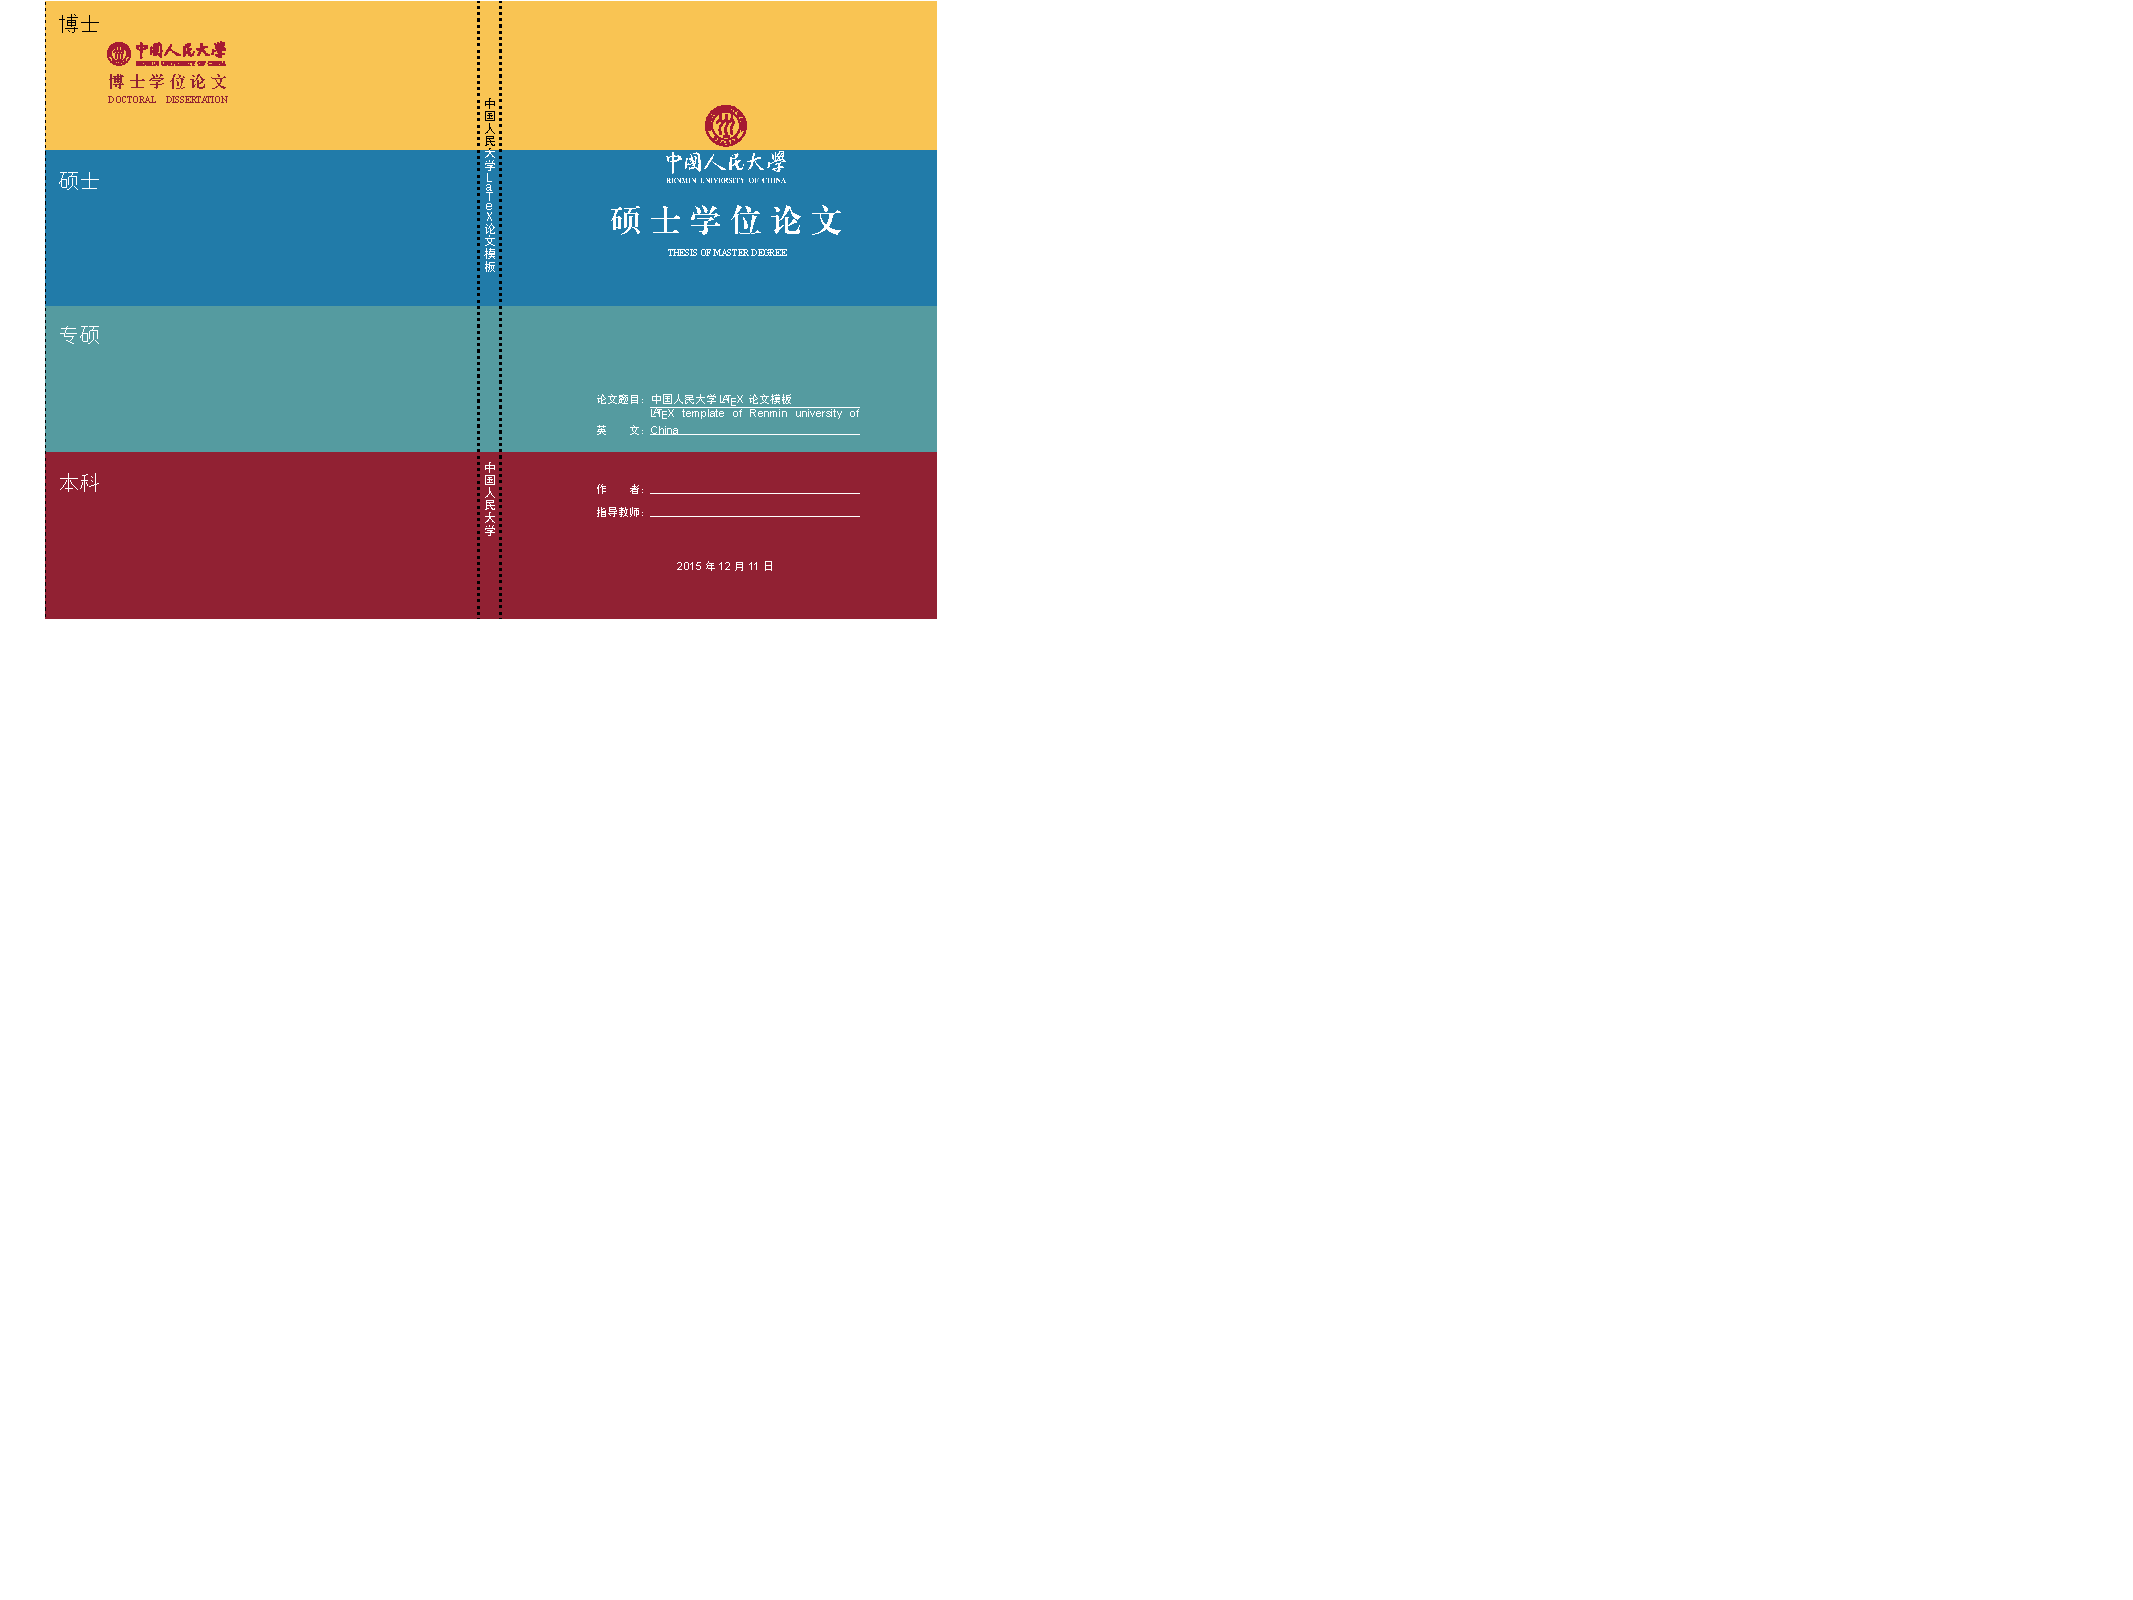
\includegraphics[width=14cm,height=9.7cm]{figures/coverpic.pdf}
\caption[cover示意图]{cover示意图}
\end{figure}